% chapter 3
\chapter{Vehicle Routing Problem}
Now that we have covered the basic concepts needed to solve the problem using LP, we shall proceed with
defining the given problem. In this section I will talk about the problem that the company DFFS face and how
we model it with vehicle routing problem model.

\section{Problem Statement}
The company DFFS is a furniture company with more than 30 stores across the UK. At one busy day, the company is scheduled to
make deliveries to 226 customers across the country. Each customers have specific demands for goods. The company has
one depot location, where it stores all of its goods for delivery and 16 delivery vans. The delivery vans only operate on
a time window from 09:00 to 17:00. On each delivery to a customer, it takes an average of 15 minutes for the workers to successfully unload the goods.
The company wants to find the routes that yield the minimum (optimal) distance and such that all customers are visited only once. They are interested
in looking at the optimal distance for both with and without the time windows.
In addition, the company wants to find out if it can use less vans to make all deliveries while keeping the distance roughly the same (or lower if possible) as
the delivery with 16 vehicles.

Modelling this problem to simulate every situations in real life can be difficult and can distract us from focusing on the core problem.
Thus, we may make the following assumptions for convenience:
\begin{enumerate}
\item The service time for all deliveries is set to 15 minutes.
\item All vans are homogeneous and have very large capacity (up to 50 items).
\item All customers have homogeneous demand of 1 item.
\item The delivery vehicles are based in a single depot.
\item The cost of function is set to distance travelled by the vans.
\item Distance from one point to another may be calculated using the haversine formula\footnote{Refer to wikipedia for this}.
\item Traffic conditions are negligible.
\end{enumerate}

\section{Problem Definition}
The problem mentioned above is also known as the vehicle routing problem (VRP), a classic optimisation problem that has been
documented and researched for decades. VRP is a problem where a fleet of vehicles, which are based on a central location (also known
as the depot), are required to visit geographically dispersed customers to fulfil their respective requirements. The main objective is
to find the optimal routes for the fleet of vehicles that yield a minimum cost, which could be in terms of fuel, time or distance.
There are many variants of VRP and they are based on the constraints imposed onto them. A few examples include VRP with multiple depot (MDVRP) and
a VRP where the customers can demand or return services (VRPB).
\begin{figure}[!ht]
  \centering
    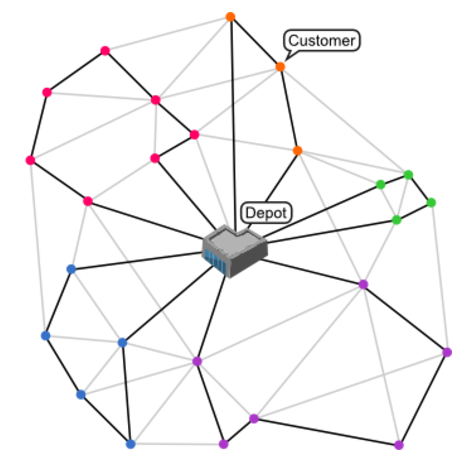
\includegraphics[width=0.6\textwidth]{vrp-sample.png}
    \caption{a visualisation of VRP}
\end{figure}

We can specifically define the problem given in the previous section with two known VRP models: capacitated
vehicle routing problem (CVRP) and capacitated vehicle routing problem
with time windows model (CVRPTW). Both of which have only one depot. The CVRP model has the following input:
\begin{itemize}
\item A complete graph \(G = (V, E)\). which consists of the vertices \(V\) and the edges \(E\).
\item The variable \(n\), which represent the total number of customers and the depot.
\item The variable \(K\), which represent the total number of vehicles available.
\item A vertex set \(V\), numbered from 1 to \(n\) and vertex 1 is the depot.
\item A set of edges for \(V\).
\item The cost function \(c_{ij}\) that outputs the distance travelled from vertex i to j, where \(i,j \in V\).
\item The path function \(x_{ij}\) that outputs 1 if the path i to j is included in the current journey and 0 otherwise.
\item The capacity function \(r(S)\) that outputs the number capacity needed to serve a set of customers \(S\).
\end{itemize}

Given the input above, we can create a single depot capacitated vehicle routing problem below (needs proper alignment):

\vspace{0.5cm}

\begin{equation}
    \begin{array}{ll@{}ll}
        \text{Minimize} & \displaystyle\sum\limits_{i \in V}\sum\limits_{j \in V} c_{ij}&x_{ij} &\\
    \end{array}
\end{equation}
\begin{equation}
    \begin{array}{ll@{}ll}
        \text{Subject to}&\displaystyle\sum\limits_{i \in V}   &x_{ij} = 1,  &\forall j \in V \setminus \{1\}\\
    \end{array}
\end{equation}
\begin{equation}
    \begin{array}{ll@{}ll}
        & \displaystyle\sum\limits_{j \in V}   &x_{ij} = 1,  &\forall i \in V \setminus \{1\}\\
    \end{array}
\end{equation}
\begin{equation}
    \begin{array}{ll@{}ll}
        & \displaystyle\sum\limits_{i \in V}   &x_{1i} = K\\
    \end{array}
\end{equation}
\begin{equation}
    \begin{array}{ll@{}ll}
        & \displaystyle\sum\limits_{i \in V}   &x_{i1} = K\\
    \end{array}
\end{equation}
\begin{equation}
    \begin{array}{ll@{}ll@{}ll}
        & \displaystyle\sum\limits_{i \in S}\sum\limits_{i \in S}  &x_{ij} \leq |S| - r(S), &\forall S \subseteq V/ \{1\} , S \neq \o \\
    \end{array}
\end{equation}
\begin{equation}
    \begin{array}{ll@{}ll@{}ll}
        & x_{ij} = \{0,1\}\\
    \end{array}
\end{equation}

\vspace{1cm}

Equations (3.2) and (3.3) are constraints to ensure that all cities are visited only once, excluding the depot. Constraints (3.4) and (3.5)
impose the vehicles coming in must be equal to the vehicles coming out of the depot. Constraint (3.6) is the subtour
elimination constraint to ensure that each route taken by the vehicle is a hamiltonian cycle\footnote{refer to wikipedia for this}. Subtour elimination
is crucial in getting the right solution as blah blah blah. Subtour is a cycle that exists in the solution.. insert explanation here.... We
have to ensure that our models take into account this procedure to ensure the accuracy and optimality of the solution.
\vspace{0.5cm}
\begin{figure}[!ht]
  \centering
    \begin{subfigure}{.5\textwidth}
      \centering
        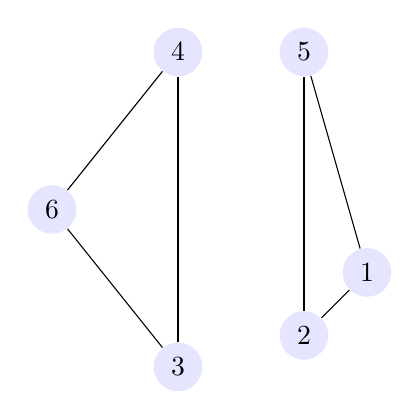
\begin{tikzpicture}
          [scale=.4,every node/.style={circle,fill=blue!10}]
          \node (n6) at (1,10) {6};
          \node (n4) at (5,15)  {4};
          \node (n5) at (9,15)  {5};
          \node (n1) at (11,8) {1};
          \node (n2) at (9,6)  {2};
          \node (n3) at (5,5)  {3};

          \foreach \from/\to in {n6/n4,n5/n1,n1/n2,n2/n5,n3/n4,n6/n3}
            \draw (\from) -- (\to);

        \end{tikzpicture}

      \caption{A subfigure}
      \label{fig:sub1}
    \end{subfigure}%
    \begin{subfigure}{.5\textwidth}
      \centering
      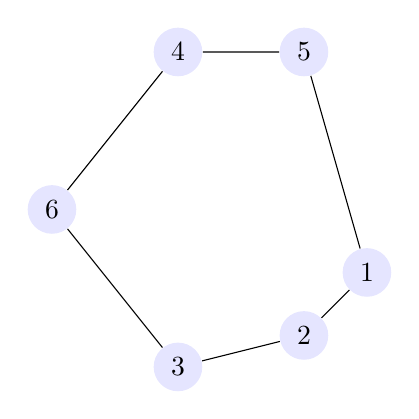
\begin{tikzpicture}
          [scale=.4,every node/.style={circle,fill=blue!10}]
          \node (n6) at (1,10) {6};
          \node (n4) at (5,15)  {4};
          \node (n5) at (9,15)  {5};
          \node (n1) at (11,8) {1};
          \node (n2) at (9,6)  {2};
          \node (n3) at (5,5)  {3};

          \foreach \from/\to in {n6/n4,n5/n1,n4/n5,n1/n2,n6/n3,n3/n2}
            \draw (\from) -- (\to);

        \end{tikzpicture}
      \caption{A subfigure}
      \label{fig:sub2}
    \end{subfigure}
    \caption{A comparison of two tours with and without subtours}
    \label{fig:test}
\end{figure}

In order to model CVRPTW, we need to introduce a new set of input related to time window constraints. We hold the assumptions made in the previous chapter.
\begin{itemize}
\item Variable \(D_{i}\) that represents the departure time to customer \(i\).
\item Time function \(t_{ij}\) that outputs the time taken to travel to customer \(i\) to \(j\).
\item Variable \(e_{i}\) that represents the earliest time for visiting customer i .
\item Variable \(l_{i}\) that represents the latest time for visiting customer i .
\item Variable \(y_{i}\) that represents the remaining capacity of the vehicle at customer \(i\) .
\item Variable \(q_{i}\) that represents the demand of customer \(i\) .
\item Variable \(Q\) that represent the capacity of the vehicle \(i\).
\end{itemize}
Putting it together, we have the complete CVRPTW model below:

\vspace{0.5cm}

\begin{equation}
    \begin{array}{ll@{}ll}
        \text{Minimize} & \displaystyle\sum\limits_{i \in V}\sum\limits_{j \in V} c_{ij}&x_{ij} &\\
    \end{array}
\end{equation}
\begin{equation}
    \begin{array}{ll@{}ll}
        \text{Subject to}&\displaystyle\sum\limits_{i \in V}   &x_{ij} = 1,  &\forall j \in V \setminus \{1\}\\
    \end{array}
\end{equation}
\begin{equation}
    \begin{array}{ll@{}ll}
        & \displaystyle\sum\limits_{j \in V}   &x_{ij} = 1,  &\forall i \in V \setminus \{1\}\\
    \end{array}
\end{equation}
\begin{equation}
    \begin{array}{ll@{}ll}
        & \displaystyle\sum\limits_{i \in V}   &x_{1i} = K\\
    \end{array}
\end{equation}
\begin{equation}
    \begin{array}{ll@{}ll}
        & \displaystyle\sum\limits_{i \in V}   &x_{i1} = K\\
    \end{array}
\end{equation}
\begin{equation}
    \begin{array}{ll@{}ll@{}ll}
        & \displaystyle\sum\limits_{i \in S}\sum\limits_{i \in S}  &x_{ij} \leq |S| - r(S), &\forall S \subseteq V/ \{1\} , S \neq \o \\
    \end{array}
\end{equation}
\begin{equation}
    \begin{array}{ll@{}ll@{}ll}
        & x_{ij} = \{0,1\}\\
    \end{array}
\end{equation}
\begin{equation}
    \begin{array}{ll@{}ll@{}ll}
        & x_{ij} = 1 \implies D_{i} + t_{ij} \leq D_{j}, \forall i, j \in V / \{1\}
    \end{array}
\end{equation}
\begin{equation}
    \begin{array}{ll@{}ll@{}ll}
        & e_{i} \leq D_{i} \leq l_{i}, \forall i \in V / \{1\}
    \end{array}
\end{equation}
\begin{equation}
    \begin{array}{ll@{}ll@{}ll}
        & x_{ij} = 1 \implies y_{i} + q_{i} \leq y_{j}, \forall i, j \in V / \{1\}
    \end{array}
\end{equation}
\begin{equation}
    \begin{array}{ll@{}ll@{}ll}
        & 0 \leq y_{i} \leq Q, \forall i \in V / \{1\}
    \end{array}
\end{equation}

\vspace{1cm}

Constraint (3.15) ensures that given a chosen path from vertex i to j, the departure time of j does not exceed the
departure time at vertex i plus the time taken to travel from vertex i to j. Constraints (3.17) and (3.18) are the
demand and capacity constraints to ensure that the capacity does not exceed the demand at any point in the given route.

\section{Solution methods for VRP}
Solution methods come in two categories: exact approaches and heuristics. Exact algorithms such as branch and bound attempts
to find the optimal solution and will not stop until it finds one of the best. On the other hand, heuristics approach
 attempts to solve a problem more quickly at the expense of optimality and precision. We use this technique in
solving many NP problems as it may take too long to compute the exact answer or when exact algorithms failed to find any exact solution.

These approaches are applied to find the solution to VRP. With larger number of vertices in VRP, it becomes more difficult
to find the exact solution. Thus, using heuristics would be convinient in this scenario. However, in smaller instances,
exact methods may be used instead.

The solvers mentioned in this project uses some of the solution methods mentioned above.

What are some of the heuristics out there?

\section{Computational Complexity}
Brief intro on P and NP hardness, and explain why VRP is np hard.

Comment on the performance of linear program against other method
... do this one later if you have time.